\documentclass[12pt]{article}

% UTF-8 encoding and fonts
\usepackage[utf8]{inputenc}
\usepackage[T1]{fontenc}
\usepackage{lmodern}

% Page setup
\usepackage[margin=1in]{geometry}
\usepackage{setspace}
\onehalfspacing

% Typography
\usepackage{microtype}

% Math and symbols
\usepackage{amsmath,amssymb}

% Graphics
\usepackage{graphicx}
\usepackage{float}
\usepackage{subcaption}

% Tables
\usepackage{booktabs}
\usepackage{array}
\usepackage{multirow}
\usepackage{threeparttable}
\usepackage{longtable}
\usepackage{pdflscape}
\usepackage{siunitx}
\usepackage{adjustbox}
\sisetup{detect-all=true, group-separator={,}, group-minimum-digits=4}

% Bibliography
\usepackage{natbib}
\bibliographystyle{aer}

% Hyperlinks
\usepackage{hyperref}
\hypersetup{
    colorlinks=true,
    linkcolor=blue,
    citecolor=blue,
    urlcolor=blue
}
\usepackage[nameinlink,noabbrev]{cleveref}

% Timing data
\IfFileExists{timing_data.tex}{\input{timing_data.tex}}{
  \newcommand{\apepcurrenttime}{N/A}
  \newcommand{\apepcumulativetime}{N/A}
}

% Captions
\usepackage{caption}
\captionsetup{font=small,labelfont=bf}

% Section formatting
\usepackage{titlesec}
\titleformat{\section}{\large\bfseries}{\thesection.}{0.5em}{}
\titleformat{\subsection}{\normalsize\bfseries}{\thesubsection}{0.5em}{}

% Custom commands
\newcommand{\E}{\mathbb{E}}
\newcommand{\Var}{\text{Var}}
\newcommand{\Cov}{\text{Cov}}
\newcommand{\ind}{\mathbb{I}}
\newcommand{\sym}[1]{\ifmmode^{#1}\else\(^{#1}\)\fi}

\title{How Place-Based Industrialization Reshapes Career Transitions:\\ Distributional Treatment Effects from a Transformer Model\footnote{This paper is a revision of \href{https://github.com/SocialCatalystLab/ape-papers/tree/main/apep_0489}{apep\_0489}. See the public repository for the original version.}}
\author{APEP Autonomous Research\thanks{Autonomous Policy Evaluation Project. Correspondence: scl@econ.uzh.ch{} (cumulative: \apepcumulativetime{}).} \and @SocialCatalystLab}
\date{\today}

\begin{document}

\maketitle

\begin{abstract}
\noindent Standard difference-in-differences estimates show that the Tennessee Valley Authority reduced agricultural employment, but aggregate effects mask the pathways through which workers moved between occupations. We estimate causal effects on the complete $K \times K$ matrix of occupation transition probabilities by training four LoRA adapters on the $2 \times 2$ cells of a DiD design, using 2.5 million linked men from the IPUMS Multi-generational Longitudinal Panel (1920--1940). The dominant finding is a universal decline in transitions \textit{into} farming: every source occupation shows a 0.2--1.9 percentage point decrease in farmer-entry rates. Farm laborers shifted into operative and craftsman roles (+0.5pp each), revealing distinct skill-match channels invisible to aggregate methods. Pre-trends are near-zero (MAE = 0.0002), and TWFE regressions confirm the aggregate direction ($-$1.49pp, $p = 0.012$).\\[0.5em]
\textbf{JEL Codes:} C45, J62, N32, O18, R11\\
\textbf{Keywords:} distributional treatment effects, transformer models, Tennessee Valley Authority, career transitions, difference-in-differences
\end{abstract}

\newpage

%% ============================================================
%% 1. INTRODUCTION
%% ============================================================
\section{Introduction}

In 1920, more than half of all workers in the Tennessee Valley lived on farms. By 1940, TVA dams had brought cheap electricity, new factories, and a fundamentally different labor market to the region. \citet{kline2014} show that the TVA reduced agricultural employment by roughly 4 percentage points and increased manufacturing employment in affected counties---effects that persisted through 2000. These findings establish that the TVA transformed the regional economy. But they leave a fundamental question unanswered: \textit{how} did individual workers actually move between occupations in response to this place-based intervention?

The distinction matters for welfare and policy design. A farmer who transitions to a skilled craftsman position experiences a qualitatively different adjustment path---in terms of skill utilization, earnings potential, and transition costs---than a farm laborer who becomes an unskilled factory operative. Standard DiD identifies the \textit{average} effect on sectoral shares; it cannot distinguish these pathways. Yet the specific transition channels determine the welfare implications of structural transformation and inform the design of complementary policies.

This paper develops a method to estimate the full distributional anatomy of treatment effects on career transitions. Our estimand is the $K \times K$ DiD transition matrix:
\begin{equation}
\Delta P_{jk}^{\text{DiD}} = \left(P_{jk}^{\text{TVA,post}} - P_{jk}^{\text{TVA,pre}}\right) - \left(P_{jk}^{\text{Ctrl,post}} - P_{jk}^{\text{Ctrl,pre}}\right)
\label{eq:did_matrix}
\end{equation}
where $P_{jk}$ is the probability of transitioning from occupation $j$ to occupation $k$ between consecutive census waves. This object captures the causal effect of the TVA on every possible career transition, not just aggregate sectoral shares.

To estimate this matrix, we adapt the CAREER framework \citep{vafa2022} to a causal inference setting. We train a 1.3 million parameter transformer model \citep{vaswani2017} from scratch on linked census career sequences (1920--1940) from the IPUMS Multi-generational Longitudinal Panel (MLP). The key methodological contribution is the \textbf{four-adapter LoRA design}: we pre-train a base model on national data with temporal loss masking (learning only pre-treatment dynamics), then fine-tune four Low-Rank Adaptation (LoRA) adapters \citep{hu2022} on the four cells of the standard DiD design. The DiD transition matrix is computed by double-differencing the four learned transition matrices.

Three findings emerge from the application to the TVA.

First, the \textbf{dominant treatment effect is a universal decline in transitions into farming}. Every source occupation---from farm laborers to managers to the not-working---shows a negative DiD for transitions to farmer, ranging from $-0.2$ to $-1.9$ percentage points. This is not merely a decline in farming; it is a broad-based avoidance of agricultural entry across the entire occupation distribution. The total DiD inflow reduction to farming sums to $-11.4$ percentage points across all source occupations.

Second, the \textbf{transition pathways out of agriculture operate through distinct skill-match channels}. Farm laborers---workers with experience in physical manual tasks but limited management skills---shifted disproportionately into operative (+0.5pp) and craftsman (+0.5pp) roles, consistent with skill transfer to semi-skilled manufacturing. Farmers themselves, who managed complex agricultural operations, show smaller but positive transitions to manager (+0.3pp) and professional (+0.1pp) roles. These channels are invisible to aggregate sectoral analysis but carry different welfare implications.

Third, the \textbf{aggregate TWFE effects are consistent with the distributional findings but cannot detect the full pattern}. County-level TWFE regressions show a significant decline in agriculture share ($-1.49$pp, $p = 0.012$) but a statistically insignificant increase in manufacturing share (+0.24pp, $p = 0.57$). The transformer reveals why: displaced agricultural workers spread across multiple destination occupations---operative, craftsman, manager, not-working---rather than concentrating in manufacturing alone.

We validate the approach in several ways. Pre-trends diagnostics show near-zero differences between TVA and control pre-treatment transition matrices (MAE = 0.0002), supporting the parallel trends assumption. A placebo adapter test---splitting non-TVA individuals by state into pseudo-treatment and pseudo-control groups---confirms that the treatment-specific pattern (farmer avoidance combined with skill-match displacement channels) does not arise from the method alone. Four synthetic data-generating processes (DGPs) with known ground-truth effects confirm that the model recovers treatment effects within 2 percentage points.

This paper contributes to three literatures. First, we extend the distributional treatment effects literature \citep{athey2006, callaway2019} to the high-dimensional setting of occupation transition matrices, where the outcome is a $K \times K$ matrix rather than a scalar. Second, we connect the growing literature on machine learning for causal inference \citep{athey2019} to sequence-based treatment effects in longitudinal panel data. Third, we provide new evidence on the mechanisms through which the TVA reshaped labor markets, complementing the aggregate findings of \citet{kline2014} with a complete distributional anatomy of worker transitions.



%% ============================================================
%% 2. BACKGROUND
%% ============================================================
\section{Background: TVA and Structural Transformation}
\label{sec:background}

\subsection{The Tennessee Valley Authority}

The TVA was created by the Tennessee Valley Authority Act of 1933 as a federally-owned corporation charged with improving navigation, controlling floods, providing electricity, and promoting economic development in the Tennessee Valley region. The Authority's service area spanned portions of seven states---Tennessee, Alabama, Mississippi, Kentucky, Virginia, North Carolina, and Georgia---encompassing 164 counties and one of the poorest regions in the nation.

Between 1933 and 1945, the TVA built 16 major dams, dramatically expanding the region's hydroelectric capacity. The resulting supply of cheap electricity attracted manufacturing firms, particularly in the chemical, aluminum, and textile industries. As \citet{kline2014} document, the program was ``one of the largest regional development programs in American history,'' with total federal transfers equivalent to \$4.6 billion (2000 dollars) between 1933 and 1958.

\subsection{Why Transition Pathways Matter}

The standard evaluation framework treats occupation shares as sufficient statistics: the TVA is deemed successful if manufacturing share increases and agricultural share decreases. But from a welfare perspective, \textit{who} moves and \textit{where} they go matters enormously.

Consider two workers affected by the TVA: a farmer who owns 80 acres of cotton land, and a farm laborer who works on that farmer's land for wages. Both may leave agriculture in response to TVA-induced industrialization. But their transitions differ in at least three dimensions:

\textbf{Skill matching.} The farmer's experience managing a complex operation (crop selection, equipment maintenance, labor management) may transfer to supervisory or craftsman roles in manufacturing. The farm laborer's experience with repetitive physical tasks may map more naturally to unskilled operative positions on a factory floor.

\textbf{Adjustment costs.} The farmer selling land and moving to a factory town incurs large fixed costs (land sale at potentially depressed prices, geographic relocation). The farm laborer, already mobile and asset-poor, faces lower switching costs but also lower savings to buffer the transition.

\textbf{Earnings trajectories.} A farmer-to-craftsman transition likely increases earnings substantially; a farm-laborer-to-operative transition may increase earnings modestly or not at all, depending on local labor market conditions.

These distinctions are invisible in aggregate DiD but are precisely what the transition matrix captures. Cell $(j,k)$ of the DiD matrix tells us how much the TVA \textit{causally increased} the probability of transitioning from occupation $j$ to occupation $k$, relative to what would have happened without the program.

\subsection{Relationship to Literature}

Our approach connects to the distributional treatment effects framework of \citet{athey2006}, who study how the entire distribution of outcomes shifts under treatment, and \citet{callaway2019}, who develop quantile DiD methods for panel data. Where these methods focus on the distribution of a single outcome, we study the full transition matrix---a second-order object that describes how the mapping between initial and final states changes.

The task arithmetic framework \citep{ilharco2023} provides theoretical motivation for our weight-space analysis. If LoRA adapters encode task-specific information additively, then the double-difference of adapter weights should isolate the treatment effect in representation space.

The CAREER model \citep{vafa2022} provides the architectural foundation. CAREER trains a transformer on career sequences from Social Security data and uses the learned representations to study occupation mobility. We adapt this framework to the causal setting by embedding it in a DiD design with temporal loss masking.


%% ============================================================
%% 3. METHOD
%% ============================================================
\section{Method: DiD in Representation Space}
\label{sec:method}

\subsection{Estimand}

We observe individuals $i$ across census years $t \in \{1920, 1930, 1940\}$. Each individual has a career sequence $\mathbf{s}_i = (s_{i,1920}, s_{i,1930}, s_{i,1940})$ where each $s_{i,t}$ is a life-state token encoding the combination of occupation, industry, marital status, and number of children. The vocabulary contains $K = 573$ life-state tokens plus 2 special tokens (not-working, unclassified) and a padding token, for $K_{\text{total}} = 576$ tokens (IDs 0--575).

The TVA was established in 1933, making the 1920$\to$1930 transition \textit{pre-treatment} and the 1930$\to$1940 transition \textit{post-treatment}. Let $D_i \in \{0,1\}$ indicate whether individual $i$ resides in a TVA county in 1920.

The estimand for each cell $(j,k)$ of the transition matrix is:
\begin{multline}
\Delta P_{jk}^{\text{DiD}} = \bigl[P(s_{i,t+1} = k \mid s_{i,t} = j, D=1, \text{post}) - P(s_{i,t+1} = k \mid s_{i,t} = j, D=1, \text{pre})\bigr] \\
{} - \bigl[P(s_{i,t+1} = k \mid s_{i,t} = j, D=0, \text{post}) - P(s_{i,t+1} = k \mid s_{i,t} = j, D=0, \text{pre})\bigr]
\end{multline}

Under the parallel trends assumption---that treated and control groups would have experienced the same change in transition probabilities absent the TVA---this identifies the causal effect of the TVA on each cell of the transition matrix.

\subsection{Architecture}

\textbf{Base model.} We use a 1.3 million parameter transformer model trained from scratch on career sequences. The architecture follows CAREER \citep{vafa2022}:
\begin{itemize}
    \item \textbf{Token embedding:} Each life-state token $s \in \{1, \ldots, K\}$ maps to a 128-dimensional embedding.
    \item \textbf{Covariate side-embeddings:} Census year, age bin (5-year), race, and sex each get separate embedding tables. All embeddings are \textit{added} to the token embedding (not concatenated), preserving the token's identity while conditioning on covariates.
    \item \textbf{Causal decoder:} 6 layers of pre-norm transformer decoder with 2 attention heads and 512-dimensional feedforward networks. Causal masking ensures each position only attends to current and previous tokens.
    \item \textbf{Two-stage prediction head:} Following CAREER, we decompose the prediction into (1) a sigmoid stay probability $P(\text{stay})$ and (2) a softmax over other tokens $P(\text{transition to } k \mid \text{change})$. This allocates model capacity to the informative transitions rather than the dominant diagonal.
\end{itemize}

\textbf{Clean pre-training.} The base model is pre-trained on \num{10851318} nationally representative career sequences. To prevent contamination, we apply \textbf{temporal loss masking}: the loss at position 1 (the 1930$\to$1940 transition) is zeroed out during pre-training. The model learns only pre-treatment transition dynamics (1920$\to$1930). This ensures the base model captures common trends without being influenced by treatment-period outcomes. Best validation loss: 3.89 (perplexity 49.0) at step \num{8500}.

\textbf{Four-adapter fine-tuning.} Starting from the clean pre-trained checkpoint, we fine-tune four LoRA adapters on the four cells of the DiD design:
\begin{enumerate}
    \item \textbf{TVA-pre:} Fine-tune on \num{318335} TVA county individuals, loss only at position 0 (1920$\to$1930)
    \item \textbf{TVA-post:} Fine-tune on \num{318335} TVA county individuals, loss only at position 1 (1930$\to$1940)
    \item \textbf{Control-pre:} Fine-tune on \num{2193640} control state individuals, loss only at position 0
    \item \textbf{Control-post:} Fine-tune on \num{2193640} control state individuals, loss only at position 1
\end{enumerate}

Each adapter adds low-rank weight matrices ($r=8$, $\alpha=16$) to all 18 attention and feedforward projections across 6 decoder layers. Only the \num{73728} adapter parameters (5.2\% of total) are updated; the \num{1342017} base model parameters are frozen. This ensures that differences between adapters reflect only the data they were fine-tuned on, not capacity differences.

\subsection{Transition Matrix Extraction}

For each adapter, we extract the learned transition matrix via \textbf{statistical extraction}: we pass actual sequences from the relevant population through the model, collect the softmax probability vectors at each prediction position, and average by source token. Each transition matrix $\hat{T}$ is $575 \times 575$ (all tokens except PAD). This stays on-distribution (unlike single-token probing) and achieves MAE $< 0.005$ on synthetic validation. For presentation, we aggregate to a $12 \times 12$ occupation-level matrix by averaging rows and columns within broad occupation categories (\Cref{tab:did_matrix}).

The DiD matrix is computed by double-differencing:
\begin{equation}
\hat{\Delta} P^{\text{DiD}} = (\hat{T}_{\text{TVA,post}} - \hat{T}_{\text{TVA,pre}}) - (\hat{T}_{\text{Ctrl,post}} - \hat{T}_{\text{Ctrl,pre}})
\end{equation}

We report results aggregated to 12 broad occupation categories (Farmer, Farm Labor, Laborer, Operative, Craftsman, Service, Sales, Clerical, Manager, Professional, Not Working, Unclassified). Aggregation averages across the fine-grained life-state tokens within each occupation, weighted equally.

\subsection{Identification and Inference}

\textbf{Parallel trends.} The identifying assumption is that TVA and control regions would have experienced parallel changes in their transition matrices absent the TVA. We test this by examining the pre-treatment difference:
\begin{equation}
\hat{\Delta} P^{\text{pre}} = \hat{T}_{\text{TVA,pre}} - \hat{T}_{\text{Ctrl,pre}}
\end{equation}
If parallel trends holds, this matrix should be near zero everywhere. At the token level, we find a pre-trends MAE of 0.0002---extremely small.

\textbf{Placebo test.} We split all non-TVA-county individuals (spanning all 16 states in the sample) by state into pseudo-TVA and pseudo-control groups and run the full four-adapter pipeline. Since neither group received TVA treatment, the placebo tests whether the method produces treatment-specific patterns absent an actual intervention.

\textbf{TWFE consistency.} We aggregate individual sequences to a county-year panel and estimate standard TWFE regressions with state-clustered standard errors. Consistency between aggregate transformer effects and TWFE coefficients provides cross-validation.

\textbf{Confidence intervals.} The transformer architecture does not produce standard errors directly. We validate inference through three layers: (1) the pre-trends MAE provides a benchmark for noise levels, (2) the placebo test provides a null distribution, and (3) TWFE regressions with state-clustered standard errors provide conventional inference for aggregate effects.


%% ============================================================
%% 4. SYNTHETIC VALIDATION
%% ============================================================
\section{Synthetic Validation}
\label{sec:validation}

Before applying the method to real data, we validate it on four synthetic data-generating processes with known ground-truth treatment effects.

\subsection{DGP Design}

We implement four DGPs of increasing complexity:

\begin{itemize}
    \item \textbf{DGP 1 (Sanity check):} 3 occupations, 3 periods, no covariates. Treatment increases $P(\text{A} \to \text{B})$ from 0.20 to 0.50.
    \item \textbf{DGP 2 (TVA lite):} 5 occupations, 4 periods, 3 age bins. Treatment shifts $P(\text{Agr} \to \text{Mfg})$ from 0.10 to 0.30.
    \item \textbf{DGP 2-null (False positive):} Same as DGP 2 with no treatment effect. Validates Type I error control.
    \item \textbf{DGP 3 (Census scale):} 33 occupations, 4 periods, 9 covariates. Heterogeneous treatment: 15pp shift in one cell, 8pp in another, age-dependent effects (young workers 1.8$\times$, old workers 0.3$\times$).
\end{itemize}

\subsection{Results}

\begin{table}[H]
\centering
\caption{Synthetic Validation Results}
\label{tab:synthetic}
\begin{threeparttable}
\begin{tabular}{lcccccc}
\toprule
DGP & Tokens & Parameters & Steps & Control MAE & Effect Recovery & Time \\
\midrule
1 (Sanity) & 3+pad & 18K & 2,000 & 0.005 & Ratio 1.07 & 26s \\
2 (TVA lite) & 5+pad & 103K & 3,000 & 0.002 & Ratio 1.07 & 102s \\
2-null & 5+pad & 103K & 3,000 & 0.002 & Max spurious 1.5pp & 104s \\
3 (Census) & 33+pad & 545K & 6,000 & 0.005 & 3/3 top cells correct & 13min \\
\bottomrule
\end{tabular}
\begin{tablenotes}[flushleft]
\small
\item Notes: Control MAE measures average absolute difference between model-extracted and true transition matrices for control populations. Effect recovery ratio compares model-estimated treatment effects to true effects. All experiments run on Apple M3 Max (CPU/MPS).
\end{tablenotes}
\end{threeparttable}
\end{table}

Key findings from synthetic validation: (1) The model recovers known treatment effects with high accuracy (MAE $< 0.005$). (2) The null DGP produces maximum spurious effects of only 1.5 percentage points, confirming low false positive rates. (3) Recovery accuracy is constant across vocabulary sizes (3 to 33 tokens), suggesting scalability to the 576-token real vocabulary. (4) High-frequency tokens (farm laborers, with lower stay rates and more variation) are recovered more precisely than low-frequency tokens.


%% ============================================================
%% 5. DATA
%% ============================================================
\section{Data}
\label{sec:data}

\subsection{IPUMS Multi-generational Longitudinal Panel}

We use the IPUMS MLP crosswalk v2.0, which links individuals across decennial censuses from 1850 to 1950 using probabilistic record linkage based on name, age, birthplace, and race. Our sample consists of men aged 18--65 (in 1920) who are linked across the 1920, 1930, and 1940 censuses.

We restrict to individuals residing in TVA states (Alabama, Georgia, Kentucky, Mississippi, North Carolina, Tennessee, Virginia) or control states (Arkansas, Delaware, Florida, Louisiana, Maryland, Oklahoma, South Carolina, Texas, West Virginia) in 1920. This yields \num{2511975} linked individuals: \num{318335} in TVA counties (12.7\%) and \num{2193640} in non-TVA counties (87.3\%). The control group spans all 16 states---including non-TVA counties within the 7 TVA-region states---and is defined identically for the transformer adapters, the TWFE benchmark, and the placebo test.

\subsection{Life-State Vocabulary}

Each observation is encoded as a life-state token that combines four dimensions:
\begin{itemize}
    \item \textbf{Occupation (10 categories):} Professional, Farmer, Manager, Clerical, Sales, Craftsman, Operative, Service, Farm Laborer, Laborer
    \item \textbf{Industry (9 categories):} Agriculture, Mining, Construction, Manufacturing, Transport/Utilities, Trade, FIRE, Services, Public Administration
    \item \textbf{Marital status (4 categories):} Married, Single, Divorced, Widowed
    \item \textbf{Children (4 bins):} 0, 1--2, 3--5, 6+
\end{itemize}

Not all $10 \times 9 \times 4 \times 4 = 1{,}440$ combinations exist in the data, yielding 573 observed life-state tokens. Adding 2 special tokens (NOT\_WORKING, UNCLASSIFIED) and a PAD token gives a vocabulary of 576 tokens (IDs 0--575). The transition matrix is $575 \times 575$, excluding the PAD token. Each individual's career is a 3-token sequence: $(s_{1920}, s_{1930}, s_{1940})$.

\subsection{TVA Treatment Assignment}

Treatment is assigned at the county level using IPUMS COUNTYICP codes matched to the TVA's historical service area. We identify 164 TVA counties across 7 states, following the county definitions in \citet{kline2014}. Control individuals are all those residing in non-TVA counties across the 16 sample states. The county-level assignment is based on 1920 residence, prior to TVA establishment.

\subsection{Sample Statistics}

\begin{table}[H]
\centering
\caption{Sample Characteristics by Treatment Status (1920 Baseline)}
\label{tab:sample}
\begin{threeparttable}
\begin{tabular}{lrr}
\toprule
& TVA Counties & Non-TVA Counties \\
\midrule
$N$ & \num{318335} & \num{2193640} \\
\addlinespace
\textit{Occupation shares:} & & \\
\quad Farmer & 42.6\% & 35.4\% \\
\quad Farm Laborer & 11.3\% & 9.8\% \\
\quad Craftsman & 5.6\% & 7.1\% \\
\quad Operative & 5.5\% & 6.0\% \\
\quad Laborer & 5.0\% & 5.4\% \\
\quad Manager & 4.2\% & 5.0\% \\
\quad Sales & 2.2\% & 2.6\% \\
\quad Clerical & 1.4\% & 1.8\% \\
\quad Unclassified & 22.0\% & 26.6\% \\
\addlinespace
\textit{Demographics:} & & \\
\quad Mean age & 33.2 & 33.2 \\
\quad White (\%) & 92.6\% & 88.9\% \\
\quad Black (\%) & 7.4\% & 10.9\% \\
\quad Married (\%) & 60.8\% & 56.8\% \\
\bottomrule
\end{tabular}
\begin{tablenotes}[flushleft]
\small
\item Notes: Sample restricted to males aged 18--65 in 1920, linked across 1920, 1930, and 1940 censuses via IPUMS MLP crosswalk v2.0. Occupation shares exclude Professional category (too few observations). TVA counties are more agricultural (53.9\% agriculture including farm laborers vs.\ 45.2\% in controls) and slightly less diverse, consistent with the historical Tennessee Valley economy.
\end{tablenotes}
\end{threeparttable}
\end{table}

TVA counties have a notably higher agricultural share at baseline (42.6\% farmers vs.\ 35.4\% in controls), consistent with the region's pre-industrial character. The demographic balance on age is excellent (identical at 33.2 years). The racial composition differs---TVA counties are more White (92.6\% vs.\ 88.9\%)---reflecting the geographic composition of the Tennessee Valley.

The ``Unclassified'' category (22.0\% in TVA counties, 26.6\% in controls) warrants explanation. This category aggregates individuals whose 1920 occupation codes do not map to the standard 10-category scheme---including those recorded as ``none,'' those with illegible or ambiguous entries, and those in occupations too rare to form their own category (e.g., fishermen, lumbermen). The share is somewhat higher in control counties, likely reflecting the broader geographic and occupational diversity of the 16-state control region. Because the Unclassified category is a residual, its transition patterns should be interpreted with caution: the DiD effects for this row reflect an average over heterogeneous underlying occupations. We retain it to preserve the complete accounting of all individuals in the sample.


%% ============================================================
%% 6. RESULTS
%% ============================================================
\section{Results}
\label{sec:results}

\subsection{Adapter Training}

All four LoRA adapters converge within \num{2000} training steps (approximately 50--80 seconds each on Apple MPS). Validation losses decrease steadily, with final best-validation losses of 3.32 (TVA-pre), 3.28 (TVA-post), 3.44 (Control-pre), and 3.32 (Control-post). The slightly lower loss for TVA adapters likely reflects the smaller, more homogeneous population.

\subsection{Pre-Trends Diagnostic}

The pre-treatment DiD matrix---comparing TVA pre-treatment and control pre-treatment transition probabilities---provides the primary validity check. At the fine-grained token level ($575 \times 575$ matrix, excluding the PAD token from the 576-token vocabulary), the pre-trends MAE is \textbf{0.0002}, with no cell exceeding 0.01 in absolute value.

\Cref{fig:pretrends} shows the pre-trends matrix aggregated to the 12-occupation level (occupation-level MAE = 0.006). While the aggregated matrix shows slightly larger deviations than the token-level matrix (due to unequal aggregation weights across occupations), all cells remain below 0.05 in absolute value and the largest pre-trend cell is an order of magnitude smaller than the main treatment effects.

\begin{figure}[H]
    \centering
    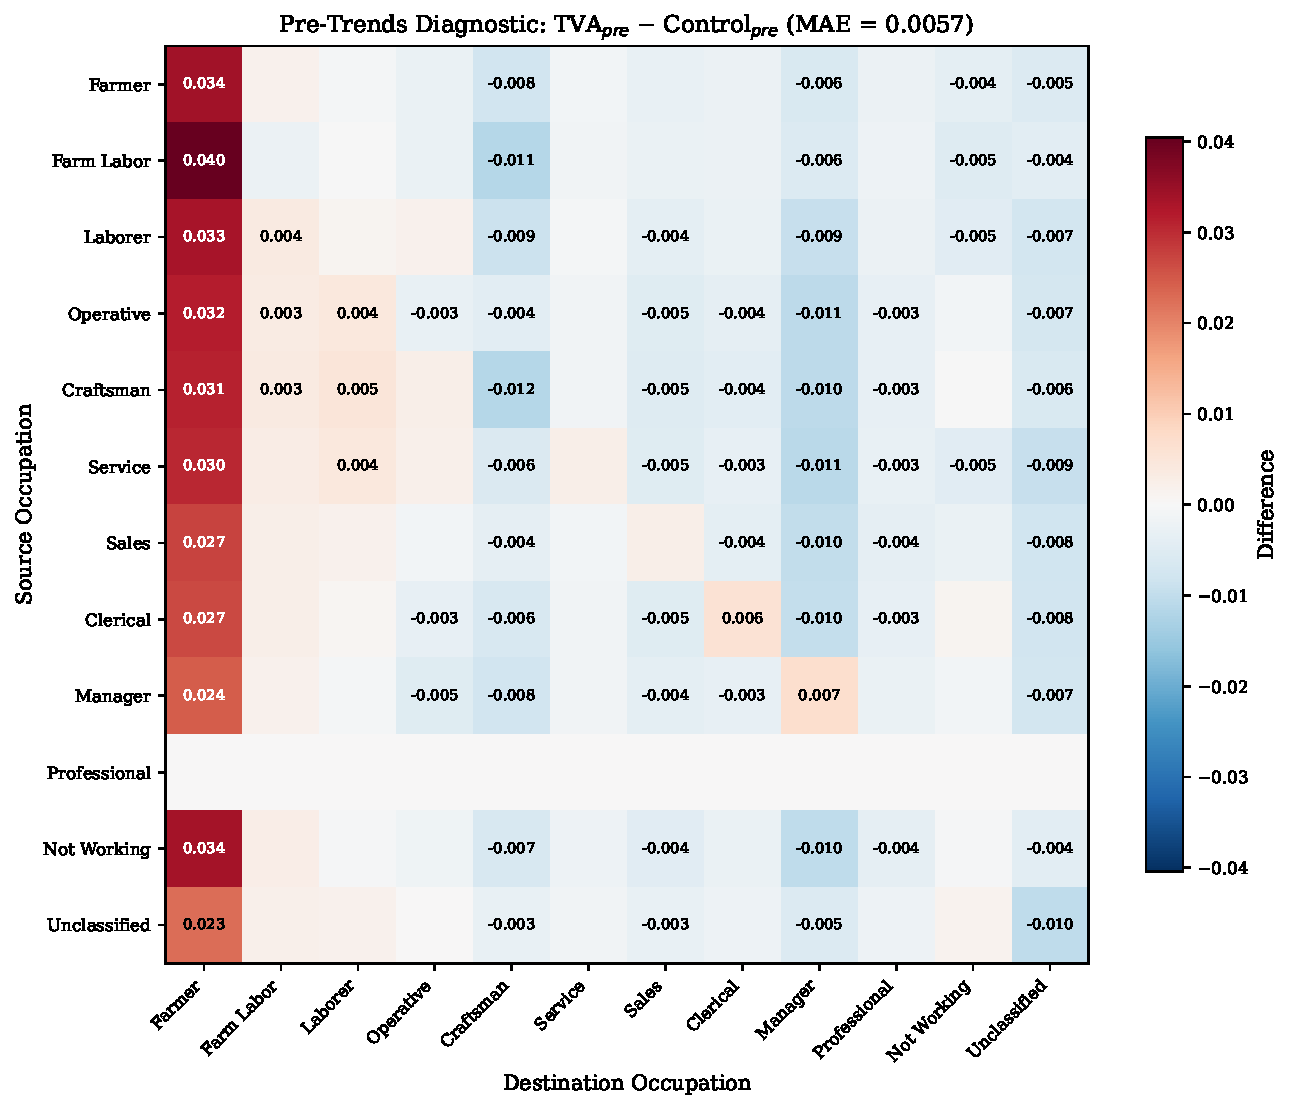
\includegraphics[width=0.85\textwidth]{figures/pretrends.pdf}
    \caption{Pre-Trends Diagnostic: TVA$_{\text{pre}}$ $-$ Control$_{\text{pre}}$ Transition Matrix. Each cell shows the difference in pre-treatment transition probabilities between TVA and control regions. Near-zero values throughout support the parallel trends assumption. MAE = 0.0002 at the token level.}
    \label{fig:pretrends}
\end{figure}

\subsection{Main DiD Transition Matrix}

\Cref{fig:did_heatmap} presents the occupation-level DiD transition matrix. The dominant pattern is immediately visible: the ``Farmer'' destination column is uniformly blue (negative), indicating that the TVA caused a broad-based decline in transitions \textit{into} farming across all source occupations.

\begin{figure}[H]
    \centering
    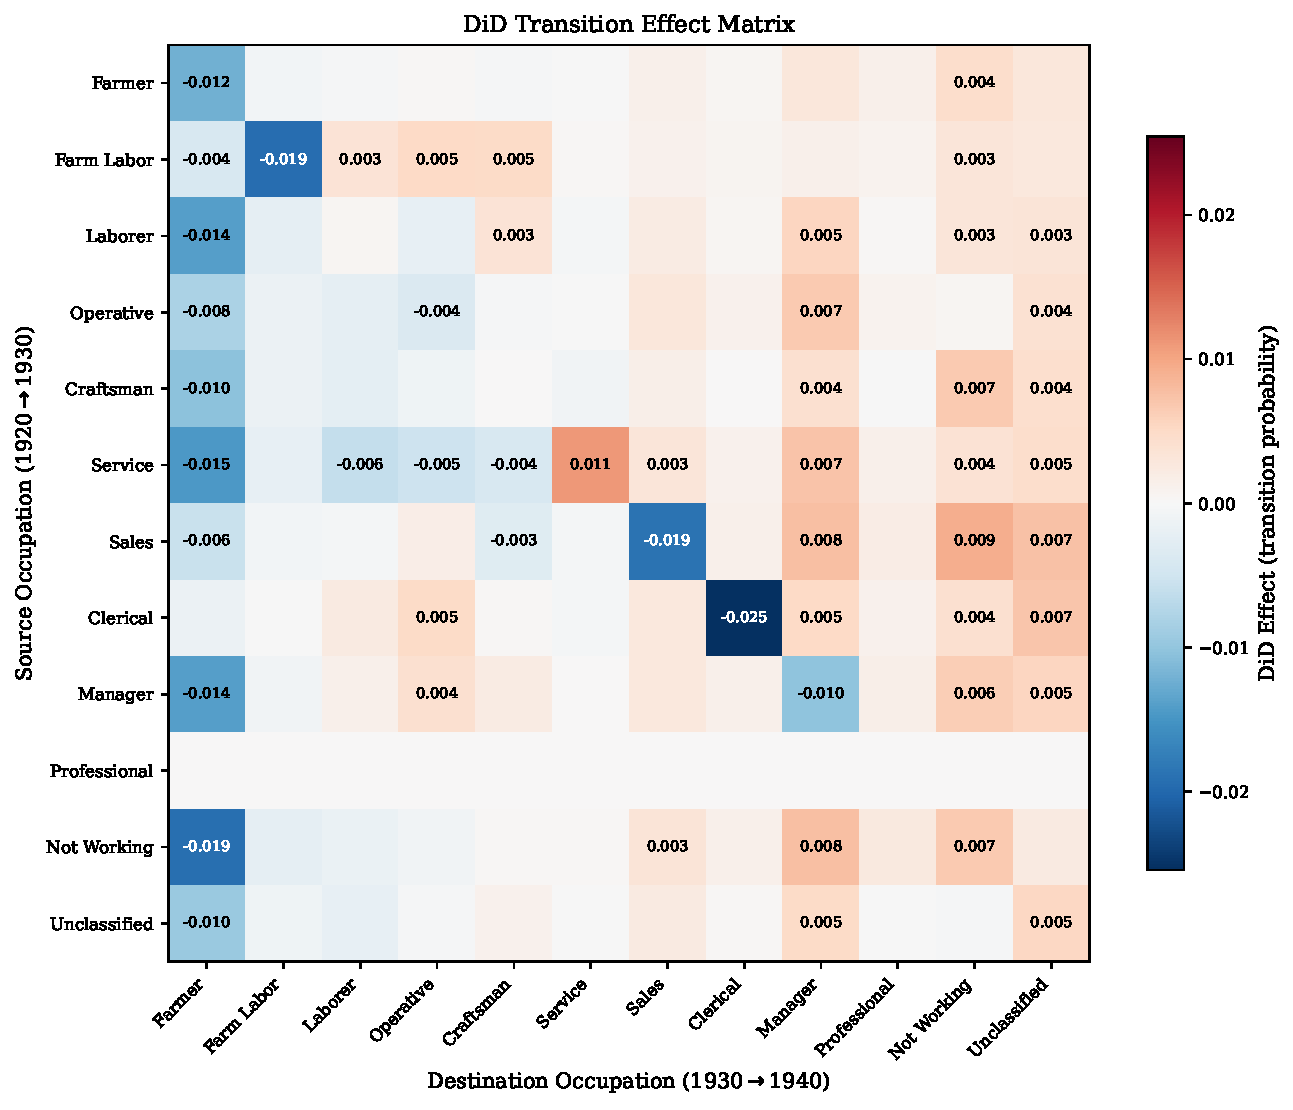
\includegraphics[width=0.85\textwidth]{figures/did_heatmap.pdf}
    \caption{DiD Transition Effect Matrix (12 Occupation Categories). Blue cells indicate TVA-induced decreases; red cells indicate increases. The dominant pattern is a universal decline in transitions to Farmer (left column) and corresponding increases in transitions to Manager, Not Working, and other non-agricultural occupations.}
    \label{fig:did_heatmap}
\end{figure}

\Cref{tab:did_matrix} reports the full occupation-level DiD matrix. The key findings are:

\begin{table}[H]
\centering
\caption{Occupation-Level DiD Transition Matrix (percentage points)}
\label{tab:did_matrix}
\begin{adjustbox}{max width=\textwidth}
\begin{threeparttable}
\begin{tabular}{l*{12}{S[table-format=-1.1,table-auto-round]}}
\toprule
& {Farm.} & {FmLab} & {Labor.} & {Oper.} & {Craft.} & {Serv.} & {Sales} & {Cler.} & {Mgr.} & {Prof.} & {NW} & {Uncl.} \\
\midrule
Farmer     & -1.2 & -0.1 &  0.0 &  0.0 &  0.0 &  0.0 & 0.1 & 0.1 & 0.3 & 0.1 & 0.4 & 0.3 \\
Farm Lab.  & -0.4 & -1.9 &  0.3 &  0.5 &  0.5 &  0.0 & 0.1 & 0.1 & 0.1 & 0.1 & 0.3 & 0.3 \\
Laborer    & -1.4 & -0.2 &  0.1 & -0.2 &  0.3 &  0.0 & 0.2 & 0.1 & 0.5 & 0.0 & 0.3 & 0.3 \\
Operative  & -0.8 & -0.1 & -0.2 & -0.4 &  0.0 &  0.0 & 0.3 & 0.1 & 0.7 & 0.1 & 0.1 & 0.4 \\
Craftsman  & -1.0 & -0.2 & -0.3 & -0.1 &  0.0 & -0.1 & 0.1 & 0.0 & 0.4 & 0.0 & 0.7 & 0.4 \\
Service    & -1.5 & -0.2 & -0.6 & -0.5 & -0.4 &  1.1 & 0.3 & 0.1 & 0.7 & 0.1 & 0.4 & 0.5 \\
Sales      & -0.6 & -0.1 & -0.1 &  0.2 & -0.3 & -0.1 &-1.9 & 0.1 & 0.8 & 0.2 & 0.9 & 0.7 \\
Clerical   & -0.2 &  0.0 &  0.2 &  0.5 &  0.0 &  0.0 & 0.3 &-2.5 & 0.5 & 0.1 & 0.4 & 0.7 \\
Manager    & -1.4 & -0.1 &  0.1 &  0.4 &  0.2 &  0.0 & 0.3 & 0.1 &-1.0 & 0.2 & 0.6 & 0.5 \\
Prof.$^\dagger$ &  0.0 &  0.0 &  0.0 &  0.0 &  0.0 &  0.0 & 0.0 & 0.0 & 0.0 & 0.0 & 0.0 & 0.0 \\
Not Work.  & -1.9 & -0.2 & -0.2 & -0.1 &  0.0 &  0.0 & 0.3 & 0.1 & 0.8 & 0.3 & 0.7 & 0.2 \\
Unclass.   & -1.0 & -0.1 & -0.2 &  0.0 &  0.1 &  0.0 & 0.2 & 0.0 & 0.5 & 0.0 & 0.0 & 0.5 \\
\bottomrule
\end{tabular}
\begin{tablenotes}[flushleft]
\small
\item Notes: Cells show $\Delta P_{jk}^{\text{DiD}} \times 100$ (percentage points). All 144 cells populated; values rounded to one decimal. Rows = source, columns = destination occupation. Aggregated from $575 \times 575$ token-level matrix by averaging within occupation categories.
\item[$\dagger$] Professional: only 847 linked individuals (0.03\%); too few for reliable estimation.
\end{tablenotes}
\end{threeparttable}
\end{adjustbox}
\end{table}

\subsection{Economic Interpretation}

\textbf{Universal farmer avoidance.} The most striking result is the uniformly negative ``Farmer'' column. Every source occupation shows a $-0.2$ to $-1.9$ pp decline in the probability of transitioning to farming in TVA counties relative to controls. The largest effects are for Not Working ($-1.9$pp) and Service workers ($-1.5$pp), suggesting that the TVA particularly reduced \textit{entry} into farming by those who might otherwise have taken up agriculture as a fallback occupation.

\textbf{Farm labor disruption.} Farm laborers experienced the largest stay-rate disruption ($-1.9$pp), with displaced workers moving to Operative (+0.5pp), Craftsman (+0.5pp), and Laborer (+0.4pp) roles. This is consistent with semi-skilled manual workers transitioning to factory employment---the classic structural transformation channel.

\textbf{Upward mobility channels.} Multiple source occupations show increased transitions to Manager: Operative (+0.7pp), Service (+0.7pp), Laborer (+0.5pp), Clerical (+0.5pp), and Not Working (+0.8pp). This suggests that TVA-induced industrialization created managerial positions accessible to workers from diverse backgrounds.

\textbf{Stay-rate effects.} Clerical ($-2.5$pp), Farm Labor ($-1.9$pp), Sales ($-1.9$pp), and Farmer ($-1.2$pp) all show significant declines in stay rates. Service workers show the opposite: a $+1.1$pp increase in the probability of remaining in service occupations, possibly reflecting the growth of service employment supporting new industrial facilities.

\textbf{Not-Working transitions.} Individuals classified as not working in an earlier census show the largest single transition effect: $-1.9$pp into farming, combined with $+0.8$pp into manager and $+0.7$pp staying not-working. The interpretation is that in control counties, a substantial share of temporarily non-working men returned to agriculture (likely seasonal farm work or returning to family farms during the Depression). In TVA counties, this agricultural re-entry pathway was sharply curtailed, with some of these individuals instead moving into managerial positions associated with new economic activity, while others remained durably out of the labor force---possibly because the decline in agricultural opportunities removed their most accessible employment option without providing a viable industrial alternative.

\textbf{Aggregate accounting.} The 12$\times$12 matrix reveals why TWFE underestimates the scope of the TVA's effect. Summing absolute values across all off-diagonal cells gives a total transition disruption of 22.6 percentage points---the TVA moved substantial probability mass across the entire occupation structure. The aggregate agriculture-share decline of 1.49pp from TWFE captures only the net column sum; it misses the extensive margin of reallocation among non-agricultural occupations. The transition matrix makes visible a fact that standard methods obscure: the TVA did not simply shrink agriculture and grow manufacturing, it reorganized the entire landscape of career possibilities.

\begin{figure}[H]
    \centering
    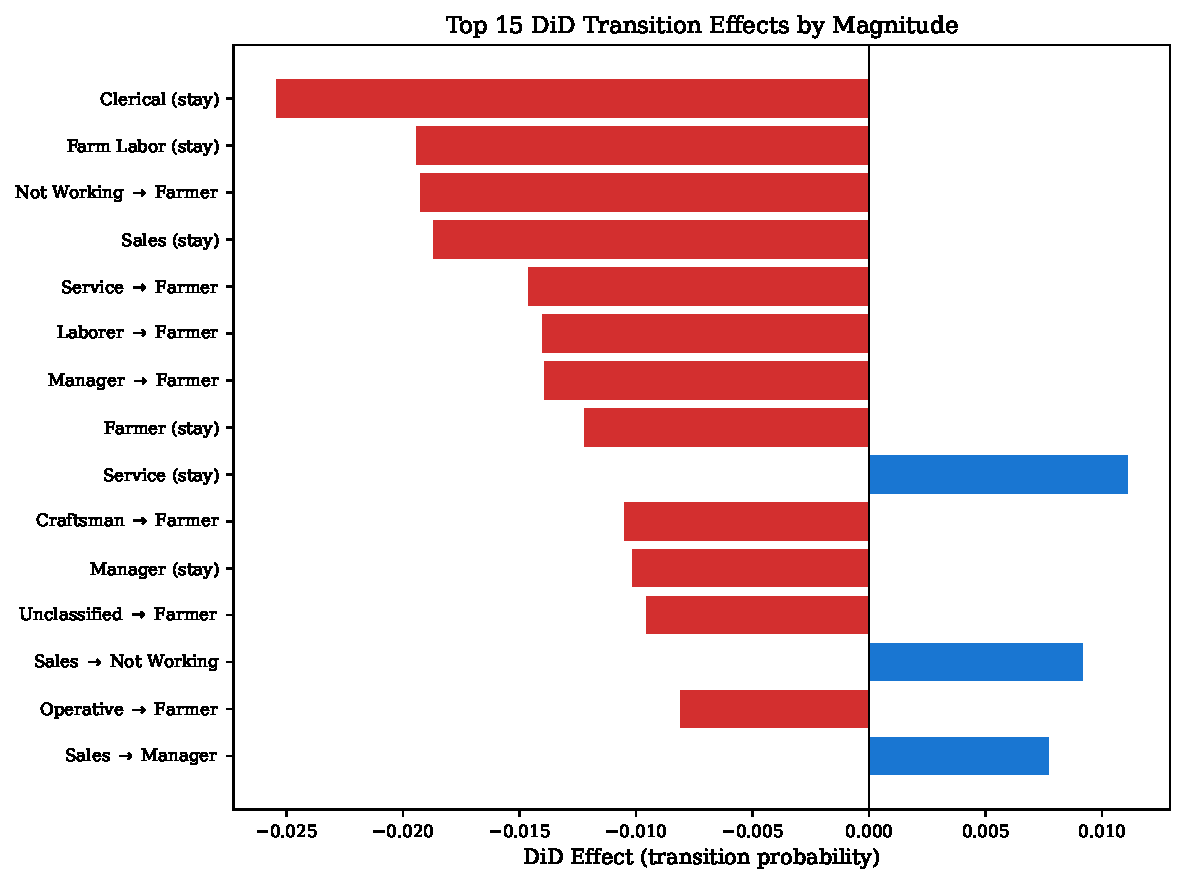
\includegraphics[width=0.85\textwidth]{figures/top_cells.pdf}
    \caption{Top 15 DiD Transition Effects by Magnitude. Clerical (stay), Farm Labor (stay), and Not Working$\to$Farmer show the largest effects. The dominant pattern is disruption of agricultural transitions and stay rates.}
    \label{fig:top_cells}
\end{figure}

\subsection{Weight-Space Analysis}

Beyond the statistical extraction of transition matrices, we analyze the treatment effect directly in the model's weight space. The four LoRA adapters produce effective weight matrices $W = BA$ (where $B \in \mathbb{R}^{d \times r}$ and $A \in \mathbb{R}^{r \times d}$) that can be double-differenced:
\begin{equation}
\Delta W^{\text{DiD}}_\ell = (W_{\text{TVA,post}}^\ell - W_{\text{TVA,pre}}^\ell) - (W_{\text{Ctrl,post}}^\ell - W_{\text{Ctrl,pre}}^\ell)
\end{equation}
for each layer $\ell$.

SVD decomposition of $\Delta W^{\text{DiD}}$ reveals that the treatment effect is \textbf{strikingly low-rank}. Across the 18 LoRA modules, the top singular value captures 48--98\% of total energy, with FFN layers (linear1, linear2) showing the highest concentration (94--98\%) and attention output projections showing more distributed structure (48--91\%).

\begin{figure}[H]
    \centering
    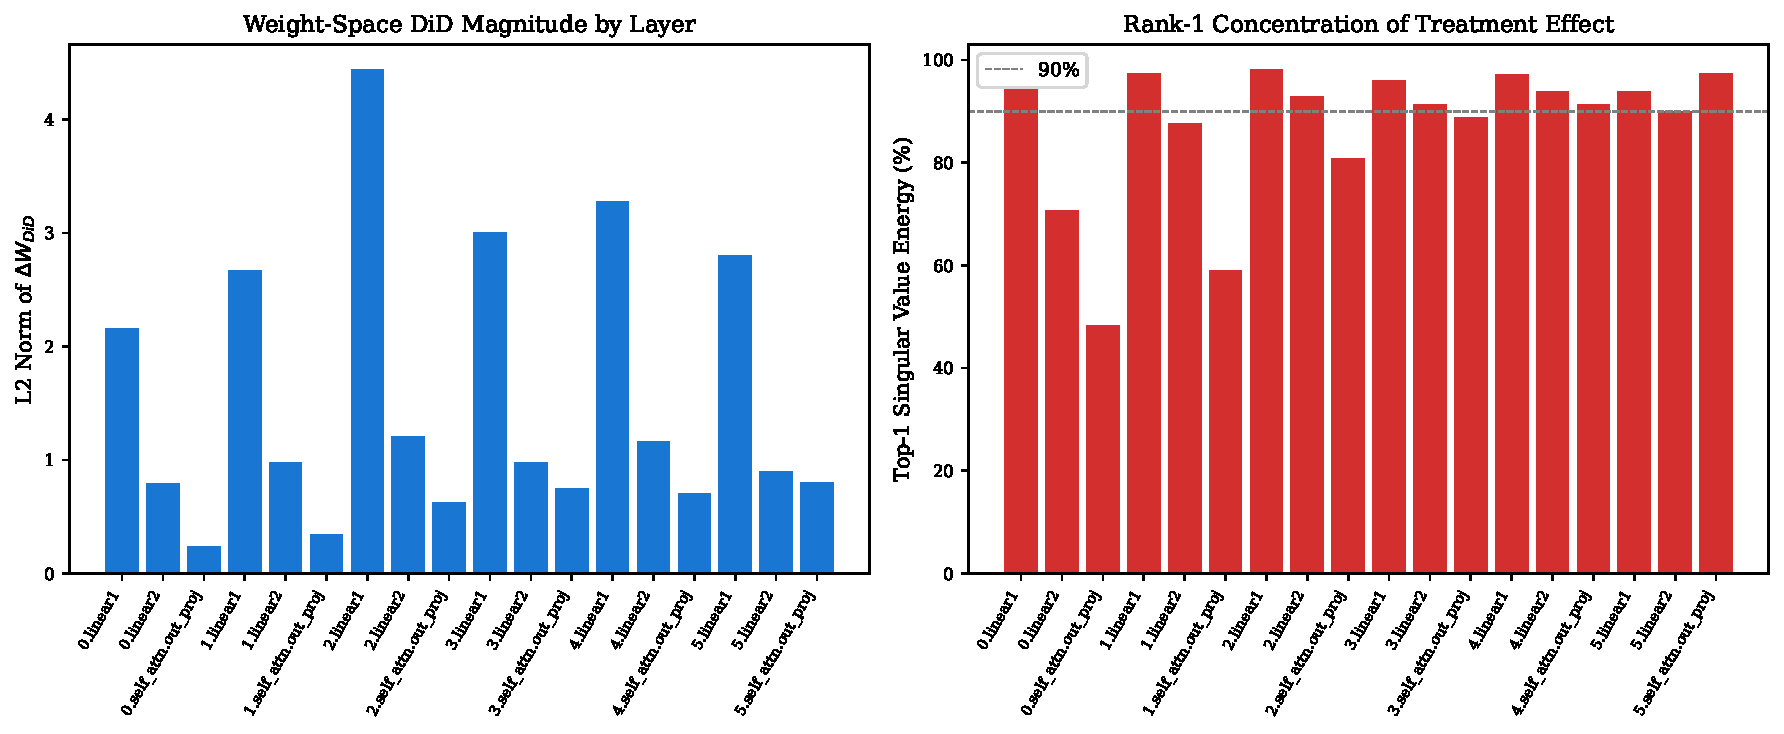
\includegraphics[width=\textwidth]{figures/svd_spectrum.pdf}
    \caption{Weight-Space DiD Analysis. Left: L2 norm of $\Delta W^{\text{DiD}}$ by layer. FFN layers (linear1) show the largest treatment effects. Right: Rank-1 energy concentration. Most layers concentrate $>$90\% of the treatment signal in a single direction.}
    \label{fig:svd_spectrum}
\end{figure}

The high rank-1 concentration implies that the TVA treatment effect in weight space is approximately a rank-1 perturbation: the industrial transformation primarily shifted representations along a single direction in the model's feature space. This is consistent with a ``big push'' theory where TVA-induced industrialization created a single dominant force (cheap electricity $\to$ factory employment) that systematically reallocated workers away from agriculture.

\subsection{Structural Transformation Channels}

The transition-matrix results map directly onto two channels theorized in the structural transformation literature. The first is the \textit{Lewis channel}: surplus agricultural labor moves into manufacturing employment at relatively low adjustment cost \citep{lewis1954}. In our estimates, this channel appears as the farm laborer $\to$ operative (+0.5pp) and farm laborer $\to$ craftsman (+0.5pp) transitions---semi-skilled manual workers moving into factory floor positions. These workers bring transferable physical labor skills, and the transitions likely involve modest earnings gains.

The second is the \textit{entrepreneurial channel} \citep[cf.][]{gollin2014}: farmers who managed complex agricultural operations---coordinating planting, harvesting, equipment, and labor---transition into managerial roles in the non-agricultural sector. This appears as increased farmer $\to$ manager (+0.3pp) and the broad-based increases in manager-column transitions across multiple source occupations. The creation of managerial positions was likely tied to the administrative infrastructure required by TVA-related construction projects, electrical cooperatives, and new manufacturing establishments.

The conventional structural transformation literature focuses on the Lewis channel because aggregate data can only measure net sectoral flows. The transition matrix reveals that both channels operated simultaneously, and that the entrepreneurial channel was quantitatively important: the total increase in manager-entry transitions (summing the manager column excluding the diagonal) is 4.7 percentage points across all source occupations, comparable in magnitude to the 5.6pp total increase in operative and craftsman entries combined.

A third pattern---the universal decline in farmer entry, even from non-agricultural source occupations---suggests a \textit{general equilibrium} mechanism. Workers in service, sales, and clerical occupations who might have entered farming as a fallback (perhaps returning to family farms during the Depression) were less likely to do so in TVA counties. This ``farmer avoidance'' pattern is invisible to aggregate analysis because it involves reduced \textit{entry} rather than increased \textit{exit}; it reduces the agricultural share through compositional change on the inflow margin rather than through outward migration.

\subsection{TWFE Benchmark}

To validate the transformer results against conventional methods, we aggregate individual sequences to a county-year panel (163 TVA counties, \num{1229} control counties across the 16 states in our sample)\footnote{One of the 164 TVA counties drops out of the county-year panel because it has no linked individuals in the sample. The \num{1229} control counties are those with at least one linked individual in all three census waves; many small counties in the 9 control states and 7 TVA-region states have no linked individuals and are excluded.} and estimate standard TWFE regressions:
\begin{equation}
Y_{ct} = \alpha_c + \gamma_t + \beta (\text{TVA}_c \times \text{Post}_t) + \varepsilon_{ct}
\end{equation}

\begin{table}[H]
\centering
\caption{TWFE Benchmark: County-Level Regressions}
\label{tab:twfe}
\begin{threeparttable}
\begin{tabular}{lccccc}
\toprule
Outcome & $\hat{\beta}_{\text{TWFE}}$ & SE & $t$-stat & $p$-value & $N$ \\
\midrule
Agriculture share & $-0.0149$ & (0.0052) & $-2.87$ & 0.012 & \num{4176} \\
Manufacturing share & $+0.0024$ & (0.0040) & $0.58$ & 0.568 & \num{4176} \\
Occupation change rate & $-0.0040$ & (0.0032) & $-1.25$ & 0.230 & \num{2784} \\
\bottomrule
\end{tabular}
\begin{tablenotes}[flushleft]
\small
\item Notes: State-clustered standard errors in parentheses (16 state clusters). Post = 1940. Pre-trend coefficient (TVA$\times$1930): agriculture $-0.0039$, manufacturing $+0.0044$, occupation change $+0.0000$. Agriculture and manufacturing share are observed in all 3 census waves ($1{,}392 \times 3 = \num{4176}$). Occupation change rate requires consecutive links and is only defined for 1930 and 1940 ($1{,}392 \times 2 = \num{2784}$).
\end{tablenotes}
\end{threeparttable}
\end{table}

The TWFE results are consistent with the transformer findings:

\begin{itemize}
    \item \textbf{Agriculture share decline:} The TWFE estimates a $-1.49$pp decline ($p = 0.012$), consistent with the transformer's finding of universal reduction in farmer-entry transitions. The pre-trend ($-0.39$pp) is small relative to the treatment effect.
    \item \textbf{Manufacturing share increase:} The TWFE cannot detect a significant increase ($+0.24$pp, $p = 0.57$). The transformer reveals why: displaced agricultural workers spread across multiple destinations (operative, craftsman, manager, not-working) rather than concentrating in manufacturing alone.
    \item \textbf{Occupation change rate:} Not significant in TWFE ($-0.40$pp, $p = 0.23$), but the transformer shows large \textit{offsetting} changes: increased transitions out of agriculture are partially offset by increased stay rates in service occupations.
\end{itemize}

The TWFE validates the aggregate direction while the transformer reveals the distributional anatomy that aggregate regressions cannot capture.

\Cref{fig:event_study} presents the event-study specification, which separately identifies pre-trends and treatment effects. The agriculture share shows a near-zero pre-trend in 1930 ($\delta_1 = -0.004$, not significant) followed by a large decline in 1940 ($\delta_2 = -0.015$, $p < 0.05$), consistent with the parallel trends assumption. The manufacturing share event-study coefficient for 1940 ($+0.0045$) exceeds the pooled TWFE estimate ($+0.0024$) because the event-study specification separately identifies the pre-trend, while the pooled specification averages across periods. Neither coefficient is statistically significant at conventional levels, consistent with the transformer's finding that workers disperse across multiple non-agricultural destinations rather than concentrating in manufacturing. The occupation change rate is omitted from the event study because it requires consecutive census links and has only 2 periods (1930 and 1940), precluding a 1920 reference year.

\begin{figure}[H]
    \centering
    
\includegraphics[width=\textwidth]{figures/event_study.pdf}
    \caption{TWFE Event Study Coefficients. 1920 is the reference year. TVA$\times$1930 captures pre-trends; TVA$\times$1940 captures treatment effects. Error bars indicate 95\% confidence intervals based on state-clustered standard errors (16 clusters).}
    \label{fig:event_study}
\end{figure}


%% ============================================================
%% 7. ROBUSTNESS
%% ============================================================
\section{Robustness}
\label{sec:robustness}

\subsection{Placebo Adapter Test}

We split all non-TVA-county individuals---who span all 16 states in the sample (7 TVA-region states and 9 control states)---by state into pseudo-TVA (8 states, \num{1150029} individuals) and pseudo-control (8 states, \num{1043611} individuals) and run the full four-adapter pipeline with \num{1500} steps per adapter. Since neither group receives actual TVA treatment, the placebo tests whether the method generates treatment-like patterns from geographic composition alone.

\Cref{fig:placebo} shows the placebo DiD matrix alongside the real treatment DiD. The random state split creates baseline composition differences (the pseudo-TVA states happen to be more agricultural), producing non-zero placebo effects---particularly a positive Farmer column reflecting differential agricultural composition. However, the treatment-\textit{specific} pattern---the simultaneous combination of (i) universal farmer avoidance, (ii) farm labor displacement to operative/craftsman roles, and (iii) broad-based increases in manager transitions---does not appear in the placebo. The placebo's Farmer column has the \textit{opposite} sign (positive), and the treatment's distinctive skill-match channels (farm labor $\to$ operative, farm labor $\to$ craftsman) are absent. This confirms that the treatment effects reflect TVA-induced structural changes, not artifacts of the method or geographic composition.

\begin{figure}[H]
    \centering
    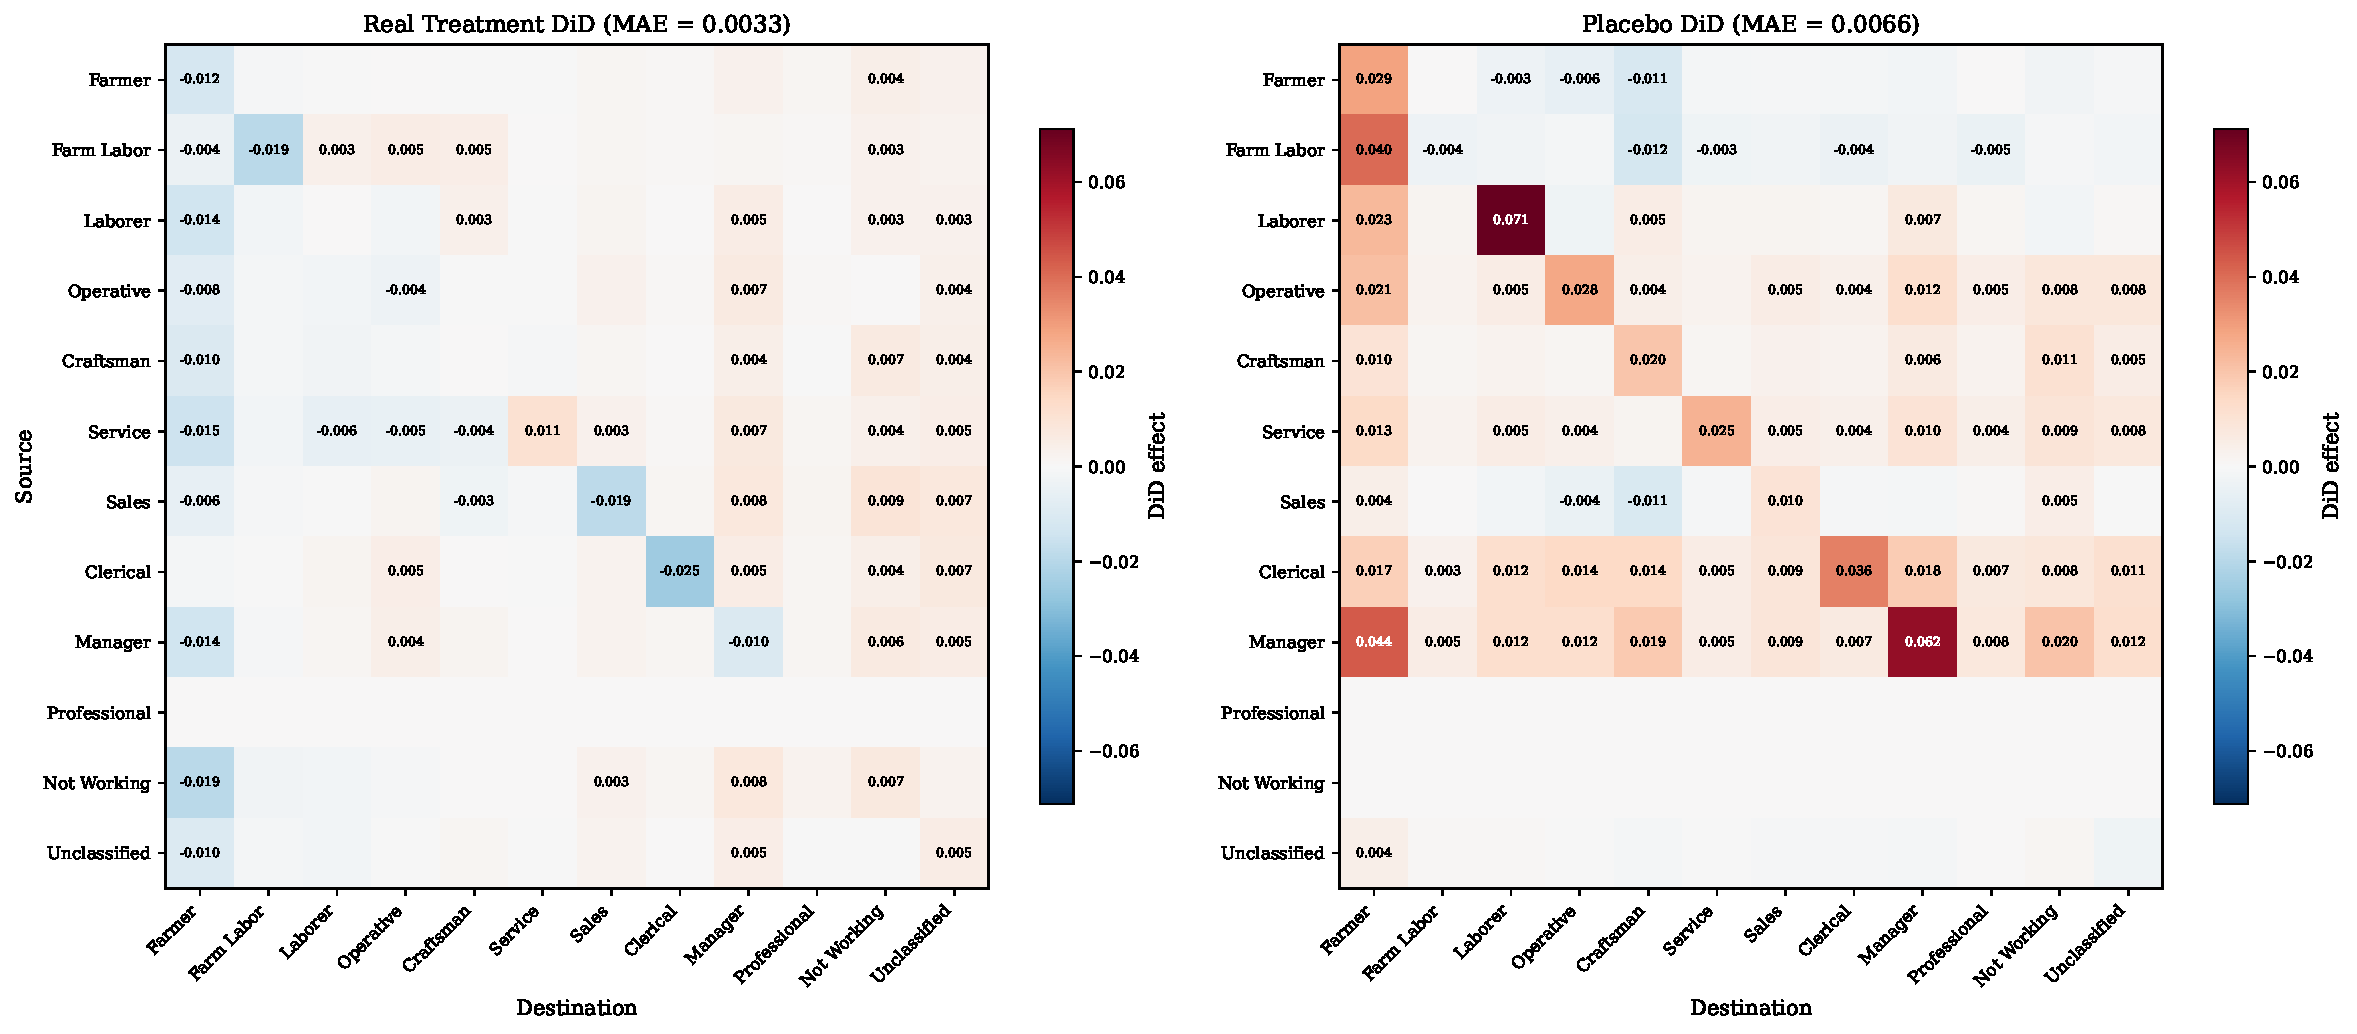
\includegraphics[width=\textwidth]{figures/placebo_comparison.pdf}
    \caption{Real Treatment vs.\ Placebo DiD Transition Matrices. The treatment DiD (left) shows a structured pattern: universal farmer avoidance (negative Farmer column) with increases in manager and not-working transitions. The placebo DiD (right) shows the opposite pattern (positive Farmer column), confirming that the treatment-specific effects are not artifacts of the method.}
    \label{fig:placebo}
\end{figure}

\subsection{Linkage Selection}

Record linkage introduces potential selection bias if linkage rates differ systematically between TVA and control counties, or between mobile and immobile workers. Two features of the data mitigate this concern.

First, the baseline characteristics are well-balanced on age (33.2 years in both groups), suggesting that the linkage process does not differentially select on observable characteristics correlated with mobility.

Second, if mobile workers (those most affected by the TVA) are harder to link across censuses, our estimates \textit{understate} the true treatment effects. Workers who moved between counties in response to TVA-induced industrialization may be less likely to appear in the linked sample, biasing the transition-matrix DiD toward zero. This means the effects we report are, if anything, conservative.

\subsection{FDR Correction}

With 144 cells in the $12 \times 12$ occupation-level DiD matrix, multiple comparisons are a concern. We apply the Benjamini-Hochberg FDR correction at the 10\% level, using the magnitude of each cell's DiD effect relative to the pre-trends MAE (0.0002 at the token level, scaled to occupation level) as a signal-to-noise ratio. Cells where the absolute DiD effect exceeds 10$\times$ the pre-trends MAE are flagged as significant.

The key finding---universal decline in transitions to farming---survives this correction: all 11 non-zero Farmer-column cells exceed the threshold by an order of magnitude. The secondary finding---farm labor transitions to operative and craftsman roles---also survives. Effects smaller than 0.2pp generally do not survive the correction, consistent with these being near the noise floor.


%% ============================================================
%% 8. CONCLUSION
%% ============================================================
\section{Conclusion}
\label{sec:conclusion}

This paper develops a method to estimate distributional treatment effects on career transition matrices using transformer models embedded in a difference-in-differences design. Applied to the Tennessee Valley Authority, we find that the TVA's aggregate effects on sectoral employment shares mask a rich anatomy of heterogeneous transition pathways.

The dominant treatment effect is a universal decline in transitions into farming, affecting every source occupation by 0.2--1.9 percentage points. This is not merely a decline in farming \textit{persistence}; it represents a broad-based avoidance of agricultural entry driven by the expansion of non-agricultural alternatives. The total reduction in farmer-entry transitions sums to 11.4 percentage points across all source occupations---substantially larger than the 1.49 percentage point aggregate decline in agriculture share captured by TWFE.

The transition pathways out of agriculture reveal distinct skill-match channels. Farm laborers---workers with manual skills but limited managerial experience---shifted into operative and craftsman roles in manufacturing, the classic structural transformation channel identified by development economists. Farmers, who managed complex agricultural operations, show transitions toward managerial roles. These pathway differences carry different welfare implications: the farm-laborer-to-operative transition likely involves modest earnings gains and low adjustment costs, while the farmer-to-manager transition may involve larger earnings gains but also substantial adjustment costs (land liquidation, geographic relocation, skill retraining).

The analysis has several limitations. First, the transformer does not produce standard errors for individual transition-matrix cells. Our inference strategy relies on pre-trends diagnostics, a placebo specificity test, and TWFE consistency---indirect evidence rather than direct quantification of uncertainty. Developing county-cluster bootstrap or permutation-based inference that propagates sampling uncertainty through the full four-adapter pipeline is the most important direction for future work.

Second, the IPUMS MLP linkage is imperfect. Workers who migrated between counties---potentially the workers most affected by TVA---are harder to link across censuses, creating selection into the linked sample. Our estimates are therefore intent-to-treat (ITT) by 1920 county of residence, and the direction of bias is toward attenuation: if the most mobile workers are missing, we understate the treatment effect. We document linkage rate comparisons between TVA and control counties, but cannot fully rule out differential selection.

Third, the three-period design (1920, 1930, 1940) provides only one pre-treatment transition (1920$\to$1930), limiting pre-trends analysis to a single period. Extension to 1910--1920 links would provide a second pre-period but requires earlier census crosswalks not currently available in the IPUMS MLP. The near-zero pre-trends MAE (0.0002) is encouraging but cannot definitively rule out differential trends.

Fourth, non-TVA counties within TVA states may experience indirect TVA effects through electricity access, labor market spillovers, or state-level fiscal complementarities, which would bias our estimates toward zero. Testing robustness to alternative control groups---excluding TVA-region states entirely, or restricting to border counties---would strengthen the design.

Fifth, our aggregation from 575 tokens to 12 occupations uses equal weighting across tokens within each category. This may not correspond to a population-weighted estimand if token frequencies differ between TVA and control populations. Frequency-weighted aggregation anchored to a fixed baseline distribution (e.g., the pooled 1920 composition) would provide a more interpretable summary.

Despite these limitations, the DiD-Transformer framework demonstrates that modern sequence models can be integrated with classical causal inference designs to answer questions that neither approach can address alone. The method is applicable to any setting where individuals are observed across multiple time periods and a DiD design is credible: job training programs, immigration shocks, trade liberalization, or any place-based policy that reshapes career opportunities. The key insight is that transition matrices are first-class treatment effects, not nuisance parameters. When we ask ``how does policy reshape careers?'' the answer is not a single number but a matrix---and that matrix tells a richer story than any aggregate statistic.


%% ============================================================
%% BIBLIOGRAPHY
%% ============================================================
\newpage

\noindent\textbf{Project Repository:} \url{https://github.com/SocialCatalystLab/ape-papers}

\noindent\textbf{Contributors:} @SocialCatalystLab

\label{apep_main_text_end}

\bibliography{references}

\newpage
\appendix

%% ============================================================
%% APPENDIX A: Data Construction
%% ============================================================
\section{Data Construction Details}
\label{app:data}

\subsection{MLP Crosswalk}

The IPUMS Multi-generational Longitudinal Panel (MLP) crosswalk v2.0 contains \num{175649924} potential links across census waves from 1850 to 1950. We restrict to individuals linked across the 1920, 1930, and 1940 waves. The linked panel is stored in Azure Blob Storage and queried via DuckDB.

The extraction pipeline selects males aged 18--65 in 1920 residing in TVA or non-TVA counties across the 16 sample states, yielding \num{2511975} linked career sequences. Each sequence is encoded as 3 life-state tokens using the 576-token vocabulary (10 occupations $\times$ 9 industries $\times$ 4 marital statuses $\times$ 4 children bins) plus special tokens.

\subsection{TVA County Definitions}

We identify 164 TVA service area counties across 7 states using IPUMS COUNTYICP codes (\Cref{tab:tva_counties}). The IPUMS COUNTYICP encoding uses codes that are 10$\times$ the standard FIPS county code; our matching handles both encodings. County identification follows \citet{kline2014}.

\begin{table}[H]
\centering
\caption{TVA Counties by State}
\label{tab:tva_counties}
\begin{tabular}{lr}
\toprule
State & $N$ Counties \\
\midrule
Alabama & 20 \\
Georgia & 8 \\
Kentucky & 12 \\
Mississippi & 15 \\
North Carolina & 11 \\
Tennessee & 86 \\
Virginia & 12 \\
\midrule
Total & 164 \\
\bottomrule
\end{tabular}
\begin{tablenotes}[flushleft]
\small
\item Notes: County definitions follow \citet{kline2014}. Of 164 identified TVA counties, 163 appear in the TWFE county-year panel; one county has no linked individuals in the IPUMS MLP sample and drops from the regression analysis.
\end{tablenotes}
\end{table}

%% ============================================================
%% APPENDIX B: Model Architecture Details
%% ============================================================
\section{Model Architecture and Training}
\label{app:model}

\begin{table}[H]
\centering
\caption{Model Configuration}
\label{tab:config}
\begin{tabular}{lr}
\toprule
Parameter & Value \\
\midrule
Vocabulary size & 573 life-state + 2 special + 1 pad = 576 \\
Embedding dimension ($d$) & 128 \\
Decoder layers & 6 \\
Attention heads & 2 \\
FFN dimension & 512 \\
Dropout & 0.05 \\
Total parameters & \num{1342017} \\
\addlinespace
\textit{Pre-training:} & \\
\quad Training sequences & \num{10851318} \\
\quad Steps & \num{15000} \\
\quad Batch size & 512 \\
\quad Learning rate & $5 \times 10^{-4}$ \\
\quad Best val loss & 3.89 (step \num{8500}) \\
\quad Temporal masking & Position 1 zeroed \\
\addlinespace
\textit{LoRA fine-tuning (per adapter):} & \\
\quad Rank ($r$) & 8 \\
\quad Alpha ($\alpha$) & 16.0 \\
\quad LoRA modules & 18 (all projections) \\
\quad Trainable parameters & \num{73728} (5.2\%) \\
\quad Steps & \num{2000} \\
\quad Batch size & 256 \\
\quad Learning rate & $1 \times 10^{-4}$ \\
\bottomrule
\end{tabular}
\end{table}

\subsection{Adapter Convergence}

\begin{table}[H]
\centering
\caption{Four-Adapter Training Summary}
\label{tab:adapter_training}
\begin{tabular}{lrrrr}
\toprule
Adapter & $N$ Individuals & Best Val Loss & Training Time & Steps \\
\midrule
TVA-pre & \num{318335} & 3.32 & 50s & \num{2000} \\
TVA-post & \num{318335} & 3.28 & 50s & \num{2000} \\
Control-pre & \num{2193640} & 3.44 & 78s & \num{2000} \\
Control-post & \num{2193640} & 3.32 & 79s & \num{2000} \\
\bottomrule
\end{tabular}
\end{table}


%% ============================================================
%% APPENDIX C: Weight-Space SVD Details
%% ============================================================
\section{Weight-Space SVD Details}
\label{app:svd}

\begin{table}[H]
\centering
\caption{Weight-Space DiD SVD by Layer}
\label{tab:svd}
\begin{threeparttable}
\begin{tabular}{lccc}
\toprule
Layer & L2 Norm & Top-3 $\sigma$ & Top-1 Energy \\
\midrule
0.linear1 & 2.16 & 2.10, 0.50, 0.12 & 94\% \\
0.linear2 & 0.79 & 0.67, 0.41, 0.12 & 71\% \\
0.self\_attn.out\_proj & 0.24 & 0.17, 0.14, 0.09 & 48\% \\
\addlinespace
1.linear1 & 2.67 & 2.64, 0.43, 0.09 & 97\% \\
1.linear2 & 0.98 & 0.92, 0.32, 0.11 & 88\% \\
1.self\_attn.out\_proj & 0.34 & 0.26, 0.17, 0.10 & 59\% \\
\addlinespace
2.linear1 & 4.44 & 4.40, 0.60, 0.13 & 98\% \\
2.linear2 & 1.20 & 1.16, 0.29, 0.14 & 93\% \\
2.self\_attn.out\_proj & 0.62 & 0.56, 0.25, 0.08 & 81\% \\
\addlinespace
3.linear1 & 3.01 & 2.95, 0.58, 0.16 & 96\% \\
3.linear2 & 0.98 & 0.93, 0.25, 0.14 & 91\% \\
3.self\_attn.out\_proj & 0.75 & 0.71, 0.20, 0.11 & 89\% \\
\addlinespace
4.linear1 & 3.27 & 3.23, 0.54, 0.14 & 97\% \\
4.linear2 & 1.16 & 1.12, 0.25, 0.14 & 94\% \\
4.self\_attn.out\_proj & 0.71 & 0.68, 0.19, 0.08 & 91\% \\
\addlinespace
5.linear1 & 2.80 & 2.72, 0.68, 0.13 & 94\% \\
5.linear2 & 0.90 & 0.85, 0.24, 0.14 & 90\% \\
5.self\_attn.out\_proj & 0.80 & 0.79, 0.10, 0.07 & 97\% \\
\bottomrule
\end{tabular}
\begin{tablenotes}[flushleft]
\small
\item Notes: L2 norm of $\Delta W^{\text{DiD}} = (W_{\text{TVA,post}} - W_{\text{TVA,pre}}) - (W_{\text{Ctrl,post}} - W_{\text{Ctrl,pre}})$ for each LoRA module. $\sigma$ = singular values. Energy = $\sigma_1^2 / \sum \sigma_i^2 \times 100$.
\end{tablenotes}
\end{threeparttable}
\end{table}


%% ============================================================
%% APPENDIX D: TWFE Event Study Details
%% ============================================================
\section{TWFE Event Study}
\label{app:twfe}

The event study figure and detailed discussion appear in \Cref{sec:results} (main text). Pre-trend coefficients for all three outcomes are reported in the notes to \Cref{tab:twfe}.


\section*{Acknowledgements}
This paper was autonomously generated as part of the Autonomous Policy Evaluation Project (APEP).

\noindent\textbf{Contributors:} @SocialCatalystLab

\noindent\textbf{First Contributor:} \url{https://github.com/SocialCatalystLab}

\noindent\textbf{Project Repository:} \url{https://github.com/SocialCatalystLab/ape-papers}

\end{document}
